\section{Datasets and signal parametrization}

Although it is possible to generate a signal sample for any \kl of interest, it is computationally way too expensive to simulate these samples for every signal point in our \kl scan, expecially because it isn't necesssary. 

The key idea is we can generate the differential cross-section for any process by exchanging the parametrization for the 3 terms ( box, triangle, and interference ) that characterize the cross-section by using a set of three basis functions by solving a set of 3 linear equations.

We work through the math below for the ggF case \Sect{\ref{subsec:ggF-sig-rw}}, and a similar property holds for VBF as well, but involves solving a set of 6 differential equations.

\subsection{ggF: histogram based reweighting}
\label{subsec:ggF-sig-rw}

%\textbf{Math from my notes reading the 2018 HH comb paper}

Although \Fig{\ref{fig:ggF_feyn_dias}} shows the LO Feynman diagrams, there is a fully differential next-to-leading-order (NLO) calculation, but the terms in this calculation still break down into diagrams in the box and triangle families.
Denoting the sum of the terms in the box and triangle diagrams as $B$ and $T$, respectively.
The impact from a non-SM coupling factors comes as a multiplicative factor for the corresponding vertices, allowing us to write down a combined amplitude (parametrized by $\kappa_t$ and $ \kappa_\lambda$ as:

\begin{equation}
\mathcal{A}(\kappa_t, \kappa_\lambda) = \kappa_t^2 B + \kappa_t \kappa_\lambda T .
\end{equation}


The ggF cross section is obtained by squaring the amplitude:

\begin{align}
	\sigma(pp \rightarrow HH) = |\mathcal{A}(\kappa_t, \kappa_\lambda) |^2 = \left( \kappa_t^2 B^* + \kappa_t \kappa_\lambda T^* \right) \left( \kappa_t^2 B + \kappa_t \kappa_\lambda T \right)  \\
	= \kappa_t^4 \left[ |B|^2 + \frac{\kappa_\lambda}{\kappa_t} (B^* T + T^* B) + \left( \frac{\kappa_\lambda}{\kappa_t}  \right)^2 |T|^2 \right] .
	\label{eq:xsec-kl-kt}
\end{align}

The $\kappa_t^4$ term scales the rate of the process. The $2^{nd}$ order $\kappa_\lambda / \kappa_t $ polynomial dictates the way these diagrams interfere, so with 3 different \kl values, we can get any arbitrary \kl value.

\def\ko{\kappa_0}
To simulate full kinematic sample, consider the basis functions with $\kappa_t = 1$ and $\kappa_\lambda = 0$ (no triangle diagram), $\kappa_\lambda =1$ and a final (now arbitrary) $\kappa_\lambda = \kappa_0$.
 
Plugging these basis points into \Eq{\ref{eq:xsec-kl-kt}} we get three different differential cross-sections:
 
\begin{align}
|\mathcal{A}(1,0)|^2 &= |B|^2 \\
|\mathcal{A}(1,1)|^2 &= |B|^2 +  (B^* T + T^* B)  + |T|^2  \\
|\mathcal{A}(1,\ko)|^2 &= |B|^2 +  \ko (B^* T + T^* B)  + \ko^2 |T|^2 
\label{eq:xec-arb}
\end{align}

\def\a{|\mathcal{A}(1,0)|^2}
\def\b{|\mathcal{A}(1,1)|^2}
\def\c{|\mathcal{A}(1,\ko)|^2}

\def\x{|B|^2} 
\def\y{(B^* T + T^* B) }
\def\z{|T|^2}

Now we solve for $\x$, $\y$, and $\z$ as a function of $\a$, $\b$, and $\c$.
Define 
\begin{equation}
\begin{cases}
x = \x \\
y = \y \\
z = \z \\
\end{cases}
\qquad \text{ and } \qquad
\begin{cases}
a = \a \\
b = \b \\
c = \c \\
\end{cases}
\end{equation}

and write this as a system of linear equations: 

\begin{equation}
\begin{bmatrix} 
a \\ b \\ c
\end{bmatrix}
 = \begin{bmatrix} 
	1 & 0 & 0 \\
	1 & 1 & 1\\
	1 & \ko & \ko^2 \\
\end{bmatrix}
\begin{bmatrix} 
x \\  y \\ z
\end{bmatrix}
\qquad 
\implies
\qquad 
a = x
%
\ \text{ and } \
%
\begin{bmatrix} 
b - a \\ c-a
\end{bmatrix}
 = \begin{bmatrix} 
	1 & 1\\
	\kappa_0 & \ko^2 \\
\end{bmatrix}
\begin{bmatrix} 
y \\ z
\end{bmatrix}
\end{equation}

Taking the inverse of the matrix to solve for the remaining two terms:

\begin{equation}
\begin{bmatrix} 
y \\ z
\end{bmatrix}
 = \frac{1}{\ko (\ko - 1)} \begin{bmatrix} 
	\ko^2  & -1\\
	-\ko & 1 \\
\end{bmatrix}
\begin{bmatrix} 
b-a \\ c-a
\end{bmatrix}
\end{equation}

\begin{align}
y &=  \frac{1}{\ko (\kappa_0 - 1)} \left[  \ko^2 (b-a) - (c-a) \right] \  = - \frac{\ko+1}{\ko} a + \frac{\ko^2}{\ko (\ko - 1)} b - \frac{1}{\ko (\ko - 1)} c  \\
z &=   \frac{1}{\ko (\ko - 1)} \left[ - \ko (b-a) + (c-a)  \right]  =  \frac{1}{\ko} a - \frac{1}{\ko - 1} b +  \frac{1}{\ko (\ko - 1)} c  
\end{align}

\def\kt{\kappa_t}
\def\klm{\kappa_\lambda}

Now we are ready to plug these expressions for the box, triangle, and interference terms ($x$, $y$, and $z$) to solve for 
$\left| \mathcal{A}(\kt,\klm) \right| ^2$ 
in terms of Eq.~{\ref{eq:xsec-kl-kt}} in terms of three known cross-sections ($a$, $b$, and $c$): 

\begin{align}
\left| \mathcal{A}( \kt,\klm )\right| ^2  = & \kt^2 \bigg{[} \kt^2 \Cline[blue]{\a} \notag \\
 & + \kt \klm \left(  - \frac{\ko+1}{\ko} \Cline[blue]{\a}  + \frac{\ko^2}{\ko (\ko - 1)} \Cline[orange]{\b}  - \frac{1}{\ko (\ko - 1)} \Cline[green]{\c}   \right) \\ 
& + \klm^2 \left( \frac{1}{\ko} \Cline[blue]{\a}  - \frac{1}{\ko - 1} \Cline[orange]{\b}  +  \frac{1}{\ko (\ko - 1)} \Cline[green]{\c}   \right)   \bigg{]}  \notag
\end{align}

Shuffling to put the terms in front of the basis functions together:

\begin{equation}
\left| \mathcal{A}( \kt,\klm )\right| ^2  = \kt^2 \bigg{[} \left(\kt^2 + \frac{\klm^2}{\ko} - \frac{1+\ko}{\ko} \kt \klm  \right) \Cline[blue]{\a}  
+ \frac{\ko \kt \klm - \klm^2 }{ \ko - 1} \Cline[orange]{\b} 
+  \frac{\klm^2 - \klm \kt}{\ko (\ko - 1)} \Cline[green]{\c}   \bigg{]} .
\end{equation}

The ATLAS HH analyses use the above prescription with the last basis function as $\ko = 20$.
Also, since we don't constrain $\kt$ (since we aren't sensitive compared to the ttH analysis), we will set $\kt = 1$ in the following.
So simplifying \Eq{\ref{eq:xsec-kl-kt}} for the combination formula for our implementation: 

\begin{equation}
\left| \mathcal{A}( \klm )\right| ^2  =  \bigg{[} \left(1 - \frac{21}{20} \klm +  \frac{1}{20} \klm^2  \right) \Cline[blue]{\a}  
+ \frac{ \klm (20 - \klm) }{ 19} \Cline[orange]{\b} 
+  \frac{ \klm ( \klm - 1) }{ 380} \Cline[green]{\c}   \bigg{]} .
\label{eq:ggf-rw-basis}
\end{equation}

Although \Eq{\ref{eq:ggf-rw-basis}} is fully differential, we just use the $m_{HH}$ differential distribution to derive reweighting functions mapping from the SM ($\kappa_\lambda = 1$) to each other $\kappa_\lambda$ signal we test.
These signal reweighting functions are derived at the parton level (so before the hadronization, detector effects, and interaction with the detector), and also in the full phase space (or before the analysis cuts).
% Truth sample was Powheg Box v2, 1m truth events for deriving these functions
These \kl reweighting functions were derived with over a million truth events in the full phase space. 
This is a simplification to just take into account the \mhh performance of the fully differential cross-section, but is an advantageous one because it means we don't need to simulate three large statistics basis samples with the full detector simulation analysis chain, and instead can just use the SM sample (which had 3.8 million simulated events) to get the rest of the \kl points.
However, to check the veracity of this assumption and the validity in the phase space of the analysis, a \kl = 10 sample (with 1.9 million simulated events) was produced and passed through the whole simulation chain, and the modeling of the reconstruction level variables was checked.
\Fig{\ref{fig:ggF-sig-rw}} shows a comparison of the reweighting performance in the 4b signal region comparing the actual \kl = 10 sample. Since we sew a good closure, we moved forward with this reweighting procedure. 
The limits for $\kappa_\lambda = 10$ sample versus the reweighted $\kappa_\lambda = 10$ sample, and the agreement was at the \%-level, further justifying us moving forward with this.

For completeness, \Fig{\ref{fig:ggf-sig-rw}} also showed the SM distribution used to reweight these variables, and you can see that the reweighting errors get quite a bit larger in regions of low support for the SM distribution. For the ggF signal, these reweighting errors didn't impact the analysis, but this choice of basis functions to avoid unphysical signal templates was a more challenging task for the VBF analysis.

\begin{figure}[hbt]
    \centering
    \subfloat[Reconstructed \mhh]{
        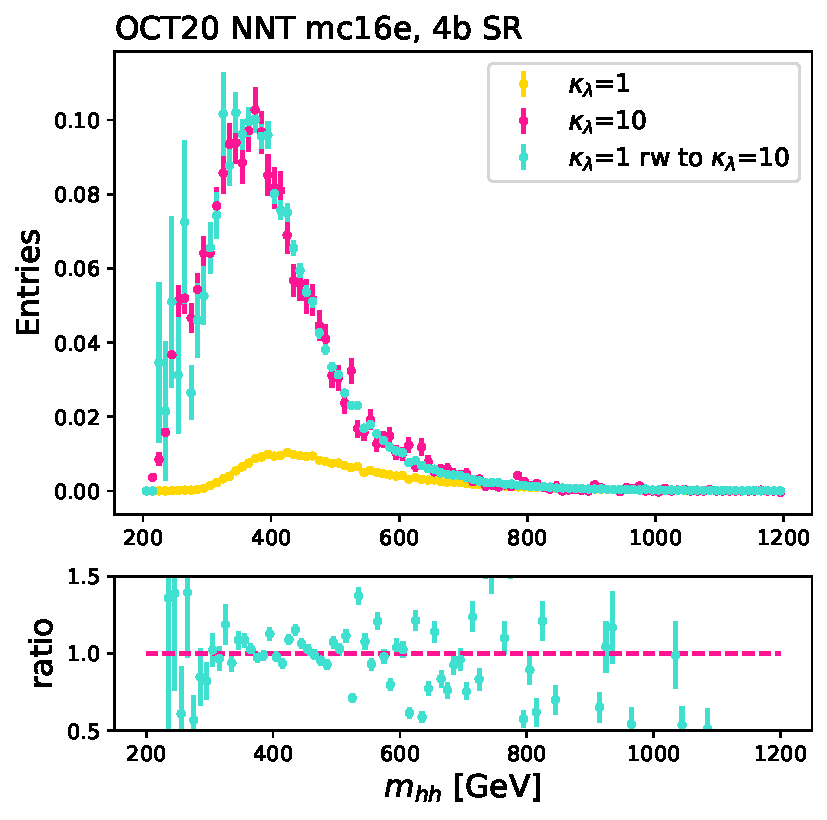
\includegraphics[width=0.45\textwidth]{{figures/my_dihiggs/m_hh_SR_4b}}
        \label{fig:ggF-sig-rw-mhh}
    }
    \subfloat[Reconstructed HH \pt]{
        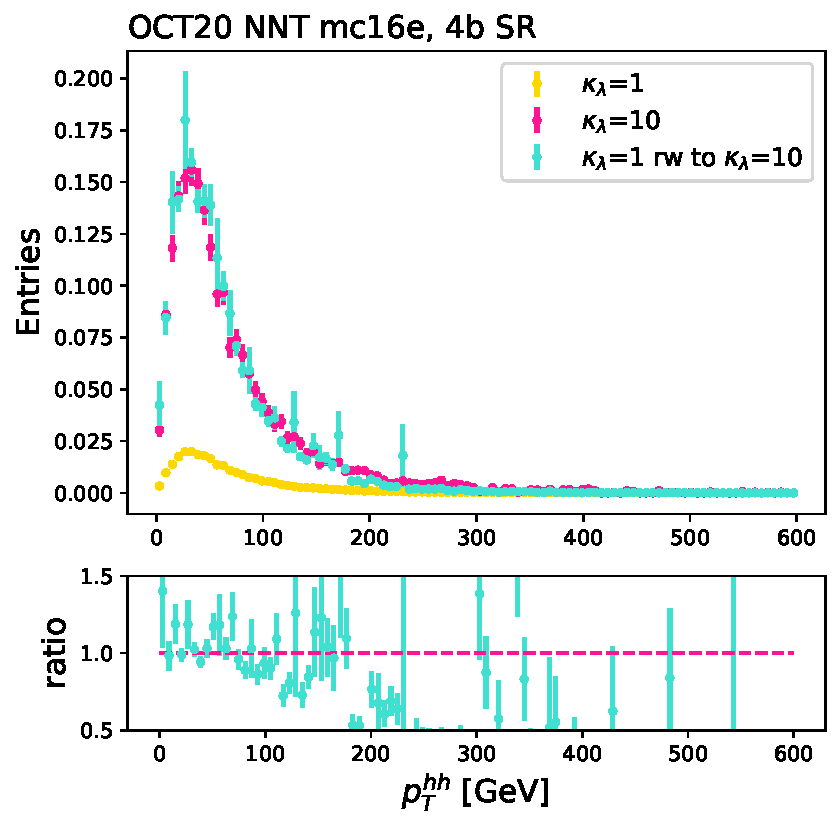
\includegraphics[width=0.45\textwidth]{{figures/my_dihiggs/pt_hh_SR_4b}}
        \label{fig:ggF-sig-rw-pthh}
    }
    \caption{Impact of the signal reweighting for the \kl=10 sample. The SM that we reweighted from is shown in yellow, while the reweighted distribution for \kl=10 is shown in turquoise and compared to the true \kl=10 distribution. \hl{Note, I'll want to include the min\_dR version of this plot instead of the BDT one}.}
    \label{fig:ggF-sig-rw}
\end{figure}

\subsection{VBF: event level reweighting}
\label{subsec:ggF-sig-rw}

For the VBF differential cross-section at arbitrary coupling values, the methodology is the same as before, except now there are three diagrams to deal with instead of two. These are shown in \Fig{\ref{fig:VBF_feyn_dias}}, where $|\mathcal{M}_\lambda|$ is the diagram that depends on \kl, $|\mathcal{M}_{2V}|$ is the diagram that depends on $\kappa_{2V}$, and $|\mathcal{M}_{V}|$ is the diagram that has two Higgses radiating separately off of the vector boson.

\def\kvv{\kappa_{2V}}
\def\kv{\kappa_V}

Writing out the differential cross-section and taking into account the scalings with respect to the couplings:

\begin{align}
\sigma(\klm, \kvv, \kv) = &\left| \kv \klm \mathcal{M}_\lambda + \kvv \mathcal{M}_{2V} + \kappa_V^2 \mathcal{M}_V \right|^2 \\
 = & \ \kv^2 \klm^2 | \mathcal{M}_\lambda |^2
 + \kv \klm \kvv ( \mathcal{M}_\lambda \mathcal{M}_{2V}^* + \mathcal{M}_\lambda^* \mathcal{M}_{2V}  )
 + \kv^3  \klm  ( \mathcal{M}_\lambda \mathcal{M}_V^* + \mathcal{M}_\lambda^* \mathcal{M}_V ) \notag \\
 &+ \kvv^2 | \mathcal{M}_{2V} |^2 
 + \kvv \kv^2 ( \mathcal{M}_{2V} \mathcal{M}_V^* + \mathcal{M}_{2V}^* \mathcal{M}_V )
 + \kv^2  |\mathcal{M}_V |^2 . \notag
 \end{align}
 
There are now 6 terms, so we can pick 6 different choices of the $(\klm, \kvv, \kv) $ couplings as basis functions to express the kinematics across the full phase space.
Although with infinite statistics we would be free to choose any 6 linearly independent couplings to find a basis, in practice with finite statistics, it's important to choose a set of basis functions that is well representative of the BSM phase space to avoid non-physical signal templates, and the corresponding choice basis samples are shown in \Tab{\ref{tab:vbf-sig-rw-basis}}.

\begin{table}[htbp]
	\centering
	\begin{tabular}{ c | c | c  }
	{\bfseries \kl} & {\bfseries $\kvv$} & {\bfseries $\kv$} \\
	\hline
	1 & 1 & 1 \\
	1 & 1.5 & 1 \\
	2 & 1 & 1 \\
	10 & 1 & 1 \\
	1 & 1 & 0.5 \\
	-5 & 1 & 0.5 
	\end{tabular}
	\caption{Coupling values defining the basis functions for the VBF signal reweighting.}
	\label{tab:vbf-sig-rw-basis}
\end{table}

Solving the system of linear equations for these basis points gives the differential cross-section for arbitrary couplings: 

% Note, it might be worth while checking this myself next time that I have the solver open
\begin{align*}
\sigma(\klm, \kvv, \kv) = \ & \left(  \frac{68}{135} \kvv^2 - 4 \kvv \kv^2 + \frac{20}{27} \kvv \kv \klm + \frac{772}{135} \kv^4 - \frac{56}{27} \kv^3 \klm + \frac{1}{9} \kv^2 \klm^2 \right) \sigma(1,1,1) \\
&+ \left( - \frac{4}{5} \kvv^2 + 4 \kvv \kv^2 - \frac{16}{5} \kv^4 \right) \sigma(1, 1.5, 1) \\
&+ \left( \frac{11}{60} \kvv^2 + \frac{1}{3} \kvv \kv^2 - \frac{19}{24} \kvv \kv \klm - \frac{53}{30} \kv^4 + \frac{13}{6} \kv^3 \klm - \frac{1}{8} \kv^2 \klm^2 \right) \sigma(2, 1, 1) \\
&+ \left(- \frac{11}{540} \kvv^2 + \frac{11}{216} \kvv \kv \klm + \frac{13}{270} \kv^4 - \frac{5}{54} \kv^3 \klm + \frac{1}{72}\kv^2 \klm^2 \right) \sigma(10, 1, 1)\\
&+ \left( \frac{88}{45} \kvv^2 - \frac{16}{3} \kvv \kv^2 + \frac{4}{9} \kvv \kv \klm + \frac{152}{45} \kv^4 - \frac{4}{9} \kv^3 \klm \right) \sigma(1, 1, 0.5)\\
&+ \left( \frac{8}{45} \kvv^2 - \frac{4}{9} \kvv \kv \klm - \frac{8}{45} \kv^4 + \frac{4}{9} \kv^3 \klm  \right) \sigma(-5, 1, 0.5)
\end{align*}
 
Although the ggF signal reweighting had good closure for just reweighting based on the truth \mhh distributions, for the VBF analysis \mhh didn't capture the full kinematics of the event that we used to define the analysis cuts and final discriminant, so the VBF signal reweighting is done at the event level using this linear combination of signal samples. 

\subsection{EFTs}
\label{subsec:EFTs}
